% !Tex root = dis.tex
\chapter{Overview of present experiment}
\graphicspath{{./images/ch3/}}

In this section I detail why certain participants are selected, which piece of software is used for the trial and why it is picked, the experimental procedure and how it relates to the research questions driving this work. At the end of this section, the reader should have the necessary background to understand the experiment.

\section{Participants}

In this study, I sought to achieve meaningful results with a 95\% confidence interval and 80\% power looking at the differences between real production code with refactoring supported by cognitive load theory principles applied and code without. I wanted to explore the difference in mean time to fix a bug, regressions introduced, and perceived cognitive load between experienced programmers and novices. Using the G*Power application [73], I computed a minimal sample size of 185 participants. For ease of calculation, I got 188.

The development practice of those who have multiple years of experience is different from those without, as is commonly seen in expert/novice studies in areas such as chess \cite{Degroot1968}, circuit analysis\cite{Egan1979}, and nursing \cite{Benner2004}. Studies in programming have explored expert schema generation and ways of reading code \cite{Ehlrich1984,Curtis1984,Rist1986}. Many of these studies have very basic modeling of programming expertise, classifying participants as experts or novices. Models such as the five stage Dreyfus Model \cite{Dreyfus1980} have not been widely applied in the research literature. Nevertheless, companies often hire programmers with criterion based on years of experience, despite the lack of a strong research body of evidence that shows correlation between expertise and years programming. For the purposes of this study, I chose to segment years of programming experience based on common industry qualifications: \textless  5 years for novices, 5+ years for experienced.

\section{Materials}

\subsection{Software Chosen - Joda Time}

For this study, I used the Joda Time date/time library. Joda is a popular open-source library used in thousands of projects for date/time manipulation for Java. Java already has a Date/Calendar library built into the language designed for these types of operations. However, many developers within the Java community were dissatisfied with the complexity of the interface Date/Calendar provides for achieving operations such as Date/Time arithmetic, time zone conversion, and formatting dates to standard formats such as ISO8601. Because of this complexity--which this research can show is a measurable difference in the cognitive load imposed by these two libraries-- Joda Time has become so popular that the author of the library was asked to completely re-write date/time handling for Java 8. 
 
\subsection{Why Joda Time?}
\begin{enumerate}
	\item Joda Time seeks to reduce the complexity of an existing interface, meaning that it has made an effort to manage the intrinsic cognitive load of date/time manipulation for users.

	\item Joda Time has a very large user base and is a high impact project within the Java community. Joda Time sits in the dependency tree of many popular software packages such as Spring, the Lift web application framework, Hibernate annotations, and many, many more. As such, this is not a contrived exercise dreamed up by a graduate student in a lab to show an effect. This is real code, battle-tested and used by millions.

	\item Joda Time is written in Java. Java and C++ are the most well-known programming languages in the community. Java is taught in many college curriculums; finding familiar programmers is less difficult than other languages. 

	\item Joda Time solves a very general problem--date \& time manipulation. Most languages have date libraries for common operations like arithmetic, formatting, or timezone conversion. Good and usable libraries provide broad, usable abstractions for complicated functionality. Date \& Time manipulation is very complicated, often causing bugs even in major professional software engineering environments. Programmers across different software engineering domains—whether they build web applications, defense contracting products, or video games—are likely to be able to “grok” it. While esoteric details of handling locale differences and nanoseconds may themselves be complex, the generality of the problem makes it more suitable for development by engineers with various backgrounds than a task such as modifying a Machine Learning library like Weka.  
\end{enumerate}
   
\subsection{What experimental intervention did I make to Joda-time?}

I used two versions of Joda Time. The control version is unmodified source from GitHub, forked from the master branch on July 24th, 2015. The experimental version applies Refactoring to the control version aligning with precepts of Cognitive Load Theory such that:
\begin{itemize}
	\item Variable identifiers are renamed for clarity
	\begin{itemize}
   		\item Clean Code: Avoid mental mappings $\rightarrow$ CLT: Integrate Explanatory Text Close to Related Visuals on Pages and Screens to Avoid Split Attention
	\end{itemize}
   	\item Each method has no more than 7+-2 lines
   	\begin{itemize}
		\item Clean Code : functions do no more than one thing $\rightarrow$ CLT: Write High Coherent Texts for Low Knowledge Readers
	\end{itemize}
	\item Methods are arranged according to their usage
	\begin{itemize}
		\item Clean Code : Newspaper Metaphor $\rightarrow$ CLT : Display Worked Examples and Completion Problems in Ways That Minimize Extraneous Cognitive Load
	\end{itemize}
	\item Each class has no more than 7+-2 methods
	\begin{itemize}
		\item Clean Code : Classes do no more than one thing $\rightarrow$ CLT: Write High 
	\end{itemize}
\end{itemize}
\subsection{What change did the participants have to make?}

Joda Time at this commit contained a bug in its parsing logic for ISO8601 dates. The ISO8601 standard is common enough to be implemented in many different programming languages and be a standard convention for transmitting dates in distributed systems. This makes the bug broadly comprehensible, have mass applicability, and a good candidate for investigation.  	
 
\subsection{Bug: ISO8601 Years}

The “devil in the detail” is all of the “edge” cases where bugs happen. One of the devilish details is the existence of a large, amorphous, ever-changing set of formats describing a date. The International Standards Organization attempted to ameliorate this with ISO8601[82], which defines a canonical format for the interchange of dates and times across locales. One of the quirks of the standard is that the published format is YYYY-MM-DD, however, the standard allows for more than 4-digit years in cases where sender and receiver have agreed upon extra digits by prepending with a + or - [$\pm$YYYYY].
Joda Time did not originally account for this. This led to the filing of the bug report:

\begin{figure}[H]
	\centering
	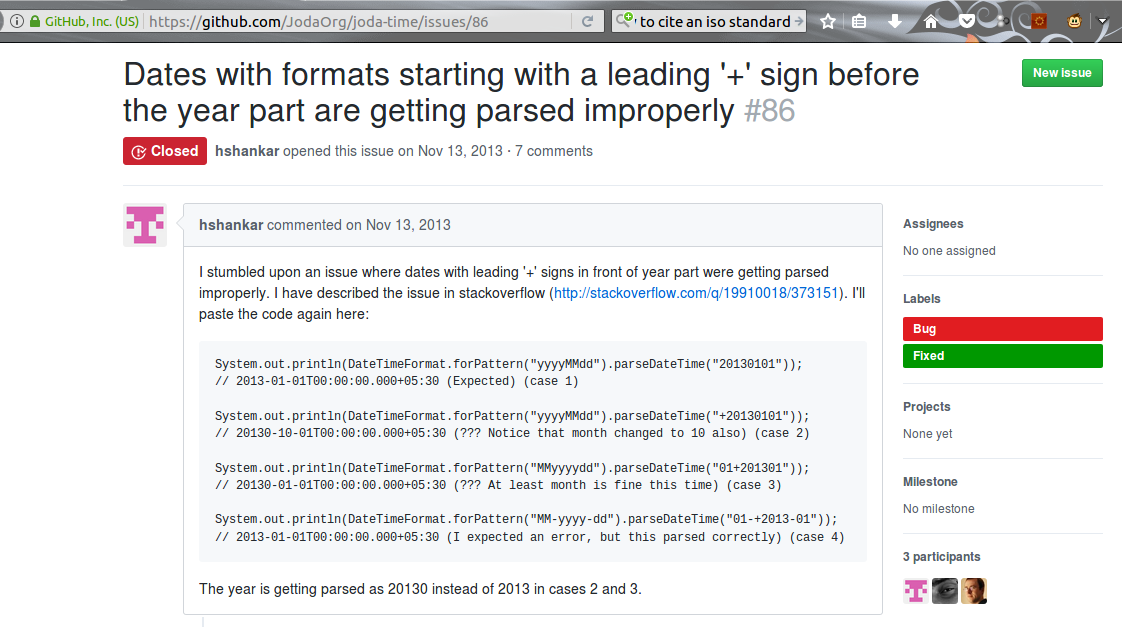
\includegraphics[width=\linewidth]{bugreport}
	\caption{insert caption}
\end{figure}

Hari Shankar explored the depths of the code, identified an issue, and made a fix. He did not report how long it took to find the bug, nor how difficult it was to come up with a solution. When I first found this issue, it was still open. 
In October of 2015, Steven Colebourne (primary author/maintainer of the library) merged in Shankar’s fix.

\begin{figure}[H]
	\centering
	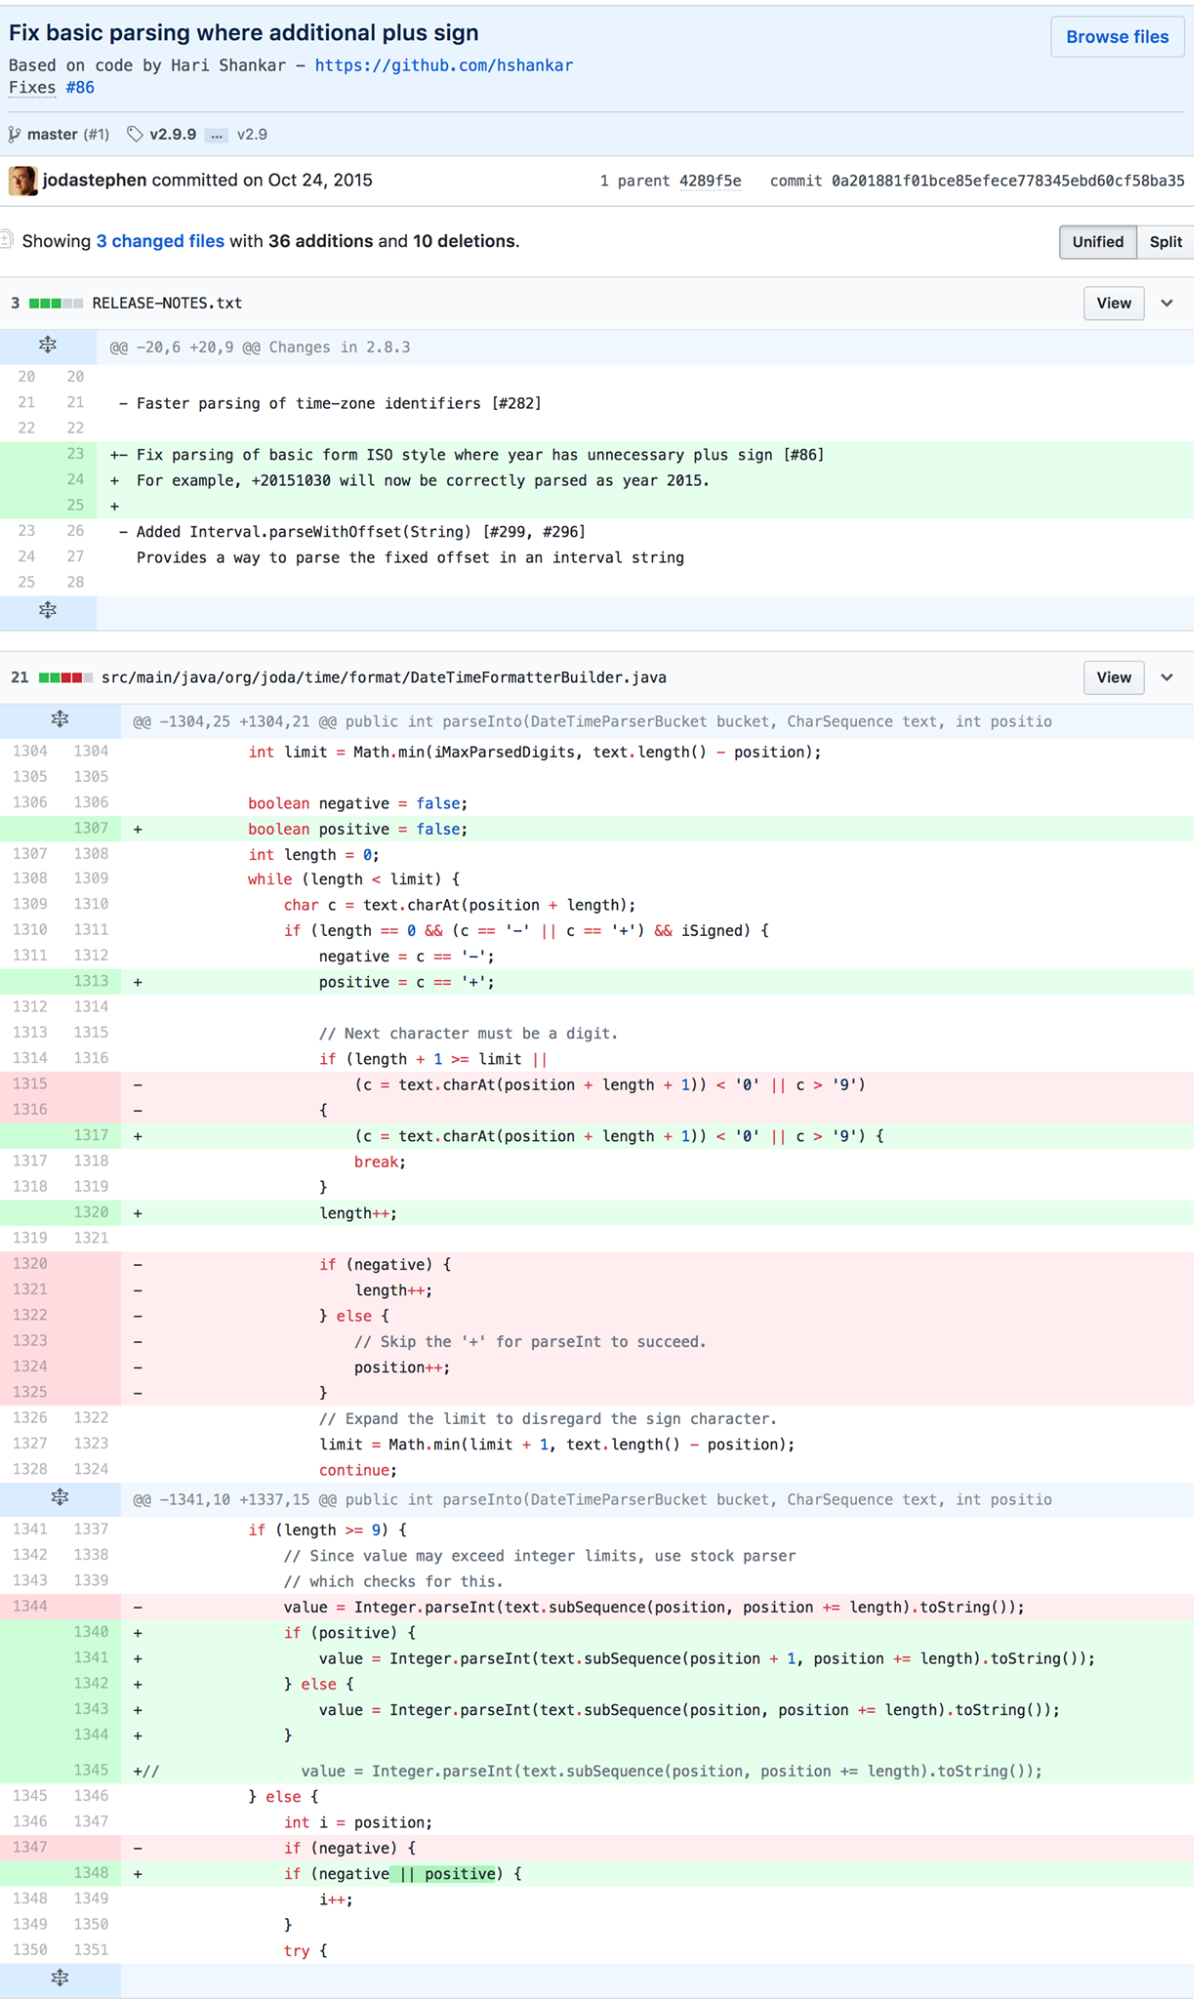
\includegraphics[height=\textheight]{Shankar'sFix}
	\caption{Shankar's Fix}
\end{figure}

\subsection{Analysis of Accepted Solution}

The accepted solution follows a common maintenance programmer practice: change as little code as possible and duplicate where necessary and with slight tweaks to achieve desired behavior. It is not exactly but similar in vein to “Programming By Difference.” It is a conservative approach that tends to be favored when code is in obsolescence, has a large number of consumers, or is otherwise hard to change.  

“Other reasons” that code can be hard to change include a lack of confidence in correct behavior, or difficulty in understanding algorithms and data structures written by someone else. The commit that introduced the fix included unit test cases that manifest the bug (though notably only try 5 digit years, perhaps not fully exercising failure modes), suggesting the maintainer understood the code enough to augment the existing test suite, a software best practice. The original code was not written solely by Stephen Colebourne. Attribution information in the comments suggests it was a collaborative effort between Colebourne, Brian S. O’Neill, and Fredrik Borgh. It’s possible this had an effect on the aggressiveness of the fix.

Using SonarQube 5.4 for analysis, I found that the \texttt{DateTimeFormatterBuilder} alone had 1600 LoC. 2625 total lines (including comments) with 162 issues found via static source analysis, with 2.3\% duplications, estimated to take 2.5 days to fix. It had a Cyclomatic Complexity score of 550, the highest in the library.

When gathering statistics of the library with the “Run Tests with Coverage” option of IDEA IntelliJ, Joda Time exhibits an impressing 98\% class/91\% line/90\% method coverage. Such a high level of coverage potentially provides developers the option to experiment with more drastic structural Refactoring and verify existing behavior, but time and other issues may not always make such re-architecture possible.	 	 

For the purposes of this experiment, I hold the state of JodaTime as reflected in Git commit on August 2nd 2015 as the “control” group, not including the given fix. I use the provided fix as the “gold standard”, as it was accepted by the core library contributor. I then ask participants to attempt to fix the bug following a short tutorial on the ISO8601 standard and the Joda Time library. I follow a 2x2 factorial design where I account for novice/expert and control/experimental measuring debugging time, number of defects introduced as detected by failing unit tests, and perceived cognitive load as reported on the Likert Scale. Non-software related factors that potentially introduce error in measurement include time of day, environmental factors in the deviation from “normal programming place” (office, coffee shop, home, et cetera) versus “clean room”, and participant mood/focus/mental factors. I treat non-software related factors as nuisance variables.

\section{Experimental Environment}
To run the study, I developed a lab machine with multiple Integrated Development Environments to suit the needs of Java programmers: Eclipse, IDEA IntelliJ, Oracle NetBeans, Sublime Text Editor, Vim, and Emacs. The lab machine included all necessary software, an Ubuntu 11.10 base OS running Java Development Kit 8 update 21, Git, installed versions of Eclipse Neon, IntelliJ IDEA 14, NetBeans 8.2, Sublime Text 3, VIM 7.1, and emacs 24.2.

This was a conscious concession to permit the introduction of another nuisance variable—IDE familiarity—into the project.

\subsection{Aside: The IDE effect}
Java developers have a lot of flexibility in the toolchain they use, limiting to one particular environment could artificially narrow the participant pool or influence the results. For example, an experienced Eclipse developer may have a significantly impaired code navigability and debugging experience in Vim, or an Emacs guru could spend valuable code investigation time instead learning the graphical user interface of IntelliJ. Making one tool mandatory could significantly deviate the sample from the programmer population, discouraging some from involvement and hamstringing the rest. I wanted to simulate the field experience of programming as closely as possible, giving participants leverage to integrate prior knowledge and work with code in their naturally preferred workflows. The trade-off is that I did observe effects where toolchain differences had an effect on the study data, including load/processing times and perspective switches of Eclipse and a stability issue with NetBeans.

The in-person approach worked effectively to pilot the study and normalize the workflow and data collection. The only problem was the time-intensiveness of the process. Since the target number of participants was 185, I needed a way of scaling out the study such that participants could independently and in isolation do the exercise in parallel. Consequently, I replicated the lab machine setup in a virtual machine image using Oracle VirtualBox 4.0. I uploaded this virtual machine image onto my website, then wrote a script with instructions sent via email to participants who registered using the online questionnaire. The virtual machine was configured to automatically record the screen and capture audio, creating a very similar experience to the in-person session. Participants would securely send me the captured video file and the filled out Likert Scale for the code listing, along with any notes that corresponded to their impressions after a debrief prompt. This development enabled my research to reach for more participants than it may otherwise have; it seems an ideal way to make a study like this capable of reaching a large number of programmers from different backgrounds all over the world.

\subsection{Cognitive Load measurement - Likert Scale}
I give participants an annotated listing (included in appendices) that applies a 7-point Likert Scale to the code listing in order to analyze perceived Cognitive Load according to common techniques.

\subsubsection*{Aside: Likert Scale construction}
Likert Scales are not commonly applied to code listings. Figuring out how to do so is a point of experimental design.
It is an expansive design space, abundant with options. Naively, one may consider applying a scale at points such as every statement/expression, every line of code, every function/method, every class definition, at package level, or even at the bundled executable/library level. I’ll discuss some of the strengths and shortcomings of this approach.

\subsubsection*{Likert Scale: every expression/statement}
A Likert Scale on every single expression or statement offers perhaps the most granular sensor for how difficult code is to understand. It’s also the most “cost prohibitive” in measurement. Any code whose full functionality that does more computation/evaluation than simple algorithms such as sum/max/min can become incredibly difficult both to instrument this way and for participants to respond. For my study, I chose “real-life production code” precisely to avoid generalized inference of programmer thought process from “toy examples”, a common critique of research into the cognitive aspects of software. As measured by SonarQube, the \texttt{DateTimeFormatterBuilder} alone has 2625 total lines, and multiple expressions or statements can be in a single line. Giving participants 5000 elements to rank assuredly biases them towards Respondent Fatigue. As this is cutting-edge research intended to establish the viability of this approach, it is absolutely imperative to minimize corruption of the data based on Respondent Fatigue.  I can ameliorate this concern by setting some axioms of things that are “easy to understand”—where one would expect the average participant to respond 1 on a 1-7 least difficult/most difficult scale.

\subsection{Minimal Cognitive Load of expressions axioms}
\begin{itemize}
	\item Declaration of a variable (e.g.  \texttt{int x};)
 	\item Assignment of a value to a variable (e.g.  \texttt{int x =  2};)
	\item Unary and Binary mathematical operations (e.g. \texttt{x++}, \texttt{x + y},\texttt{ x mod y})
\end{itemize}
These axioms are challengeable. For instance, the usage of a type in a variable declaration is programming language dependent. There may be measurable differences in simplicity of understanding declarations based on the inherent type systems of the language. The way that such affects comprehensibility may be unexpected. Perhaps in a typeless language such as Assembly, or a language that allow anonymous types/”Duck Typing” such as Javascript, var x = 4 causes respondents less Cognitive Load than int x = 4. Conversely, perhaps the Germane Cognitive Load induced by the assumptions of types such as “an Integer in Java must be a whole number between -231 to 231-1” makes the second statement easier to understand. Both of these conditions may actually be determined by the target programmer’s prior experience with programming and languages.

For another example, bit shifting of whole numeric values can be succinctly described as unary/binary mathematics operations, but that may underestimate the cognitive complexity a programmer has to compute to understand what is happening. This comes up in my study in a very concrete way, as the computation of year values during the parsing step contains expressions that befuddled many participants.

\begin{figure}[H]
	\centering
	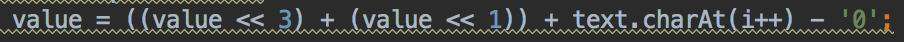
\includegraphics[width=\linewidth]{code}
	\caption{insert caption}
\end{figure}

This computation relies on a traditional programmer idiom from the assembly days, that
i*10 = (i\textless \textless 3) + (i\textless \textless1)
This shortcut is not documented in the code itself and is not one high-level application developers and other software engineers encounter on a daily basis. Every participant that encountered the line during in-person trials reported feeling uncomfortable with it. Some took the time to prove to themselves that the formula worked, many took it as given. Surely this line is not equivalent in cognitive complexity to a simple variable assignment. In these cases, I can compute a metric using Halstead’s software metrics or Mira’s Modified Cognitive Complexity Measure \cite{Choe2013}, but none of these metrics could quite capture the Cognitive Load of a prior knowledge lookup from a well-known programmer vocabulary pattern-matching schema. In principle, capturing the subjective Cognitive Load experienced by programmers encountering this line in production code could inform researchers more about the average conceptual vocabulary of programming than other mechanisms.

\subsection{Likert Scale: line-by-line}
 A Likert Scale on every single line of code is slightly less expansive than expression/statement, but not by much. Respondent Fatigue is still an overriding concern. The axioms can be expanded further to include line specific concepts.

\subsection{Minimal Cognitive Load of lines axioms}
\begin{itemize}
	\item Return statements (e.g. \texttt{return x + y};)
	\item Comments (e.g.  \texttt{// Next character must be a digit})
\end{itemize}
\subsection{Likert Scale: blocks/scopes}
This was ultimately the approach I chose to have participants respond to. Functions/Methods, classes, packages—all of these artifacts are essentially programming language conveniences to define scope at different levels of abstraction. This scope management maps very cleanly to Cognitive Load Theory’s concepts of Chunking and Sequencing. Code blocks form lexical and conceptual closures where programmers can partition their understanding of the global state of the program to management pieces. As there fewer than 100 blocks to be analyzed, I avoid the problem of Responder Fatigue but can still capture valuable granular data.

\subsection{Minimal cognitive load of blocks/scopes axioms}
\begin{itemize}
	\item Getters (e.g. \texttt{public int getCurrentPosition() \{ return currentPosition\}; })
	\item Setters (e.g. \texttt{public void setPosition(final int position) \{ this.position = position\}; })
\end{itemize}
\subsection{Open Question: How do we measure code flow cognitive complexity?}
Likert Scales at the block level get me closer, but still don’t quite capture all of the complexity programmers encounter when understanding code. For an applied example, I can examine the code flow of the \texttt{DateTimeFormatter}. The \texttt{DateTimeFormatter} uses an \texttt{InternalParser},which is implemented by a static abstract class \texttt{NumberFormatter} inside of \texttt{DateTimeFormatterBuilder}. This \texttt{NumberFormatter} is a nested class that serves as the root of an inheritance hierarchy, for classes that include \texttt{UnpaddedNumber}, \texttt{PaddedNumber}, and \texttt{FixedNumber}. Many participants who provided feedback about the design in the study expressed confusion and incredulity, some expressed outright contempt as they struggled to navigate between classes and trace control flow. This type of activity is simple to observe but difficult to capture quantitatively, and the self-reported Cognitive Load of block of code may not be able to tell us about the cognitive complexity added by interactions between the blocks. This remains an active area of potential innovation in study design and measurement for subsequent research. As a general guideline, software designers should avoid deep inheritance hierarchies or long method chains where the number of jumps in control flow begins to approach human short-term memory limits. 

The full Likert scale instrument for measuring cognitive load can be found in the appendices, here I’ll show an example question for maximum clarity:

The instrument presents some code--a method of a class-- with a 7 point scale where respondents can rank its complexity. For consistency and simplicity of data analysis, in my study this same scale is repeated for every question, only the code changes.

\begin{figure}[H]
	\centering
	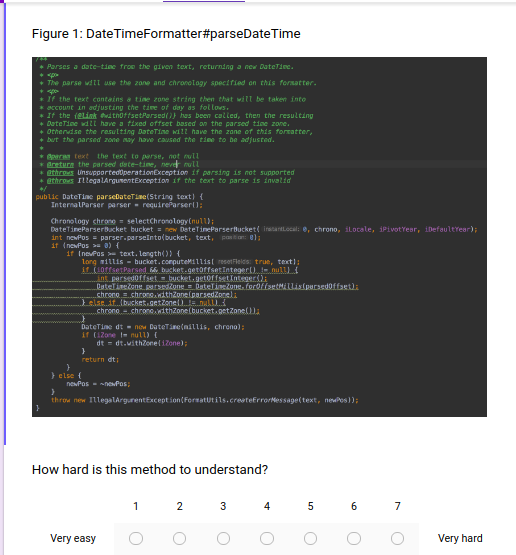
\includegraphics[width=\linewidth]{DateTimeFormatter}
	\caption{Date Time Formatter}
\end{figure}

In this section I have detailed the rationales for criterion I used to select participants, the software library I used and how I modified it for the experimental purpose, the environment developed to conduct the experiment, and the construction of the measurement instrument for cognitive load. In the next section, I’ll detail the execution of the study.   
